   \documentclass{article}
\usepackage{pgfplots}
\begin{document}
\begin{figure}
  \centering
  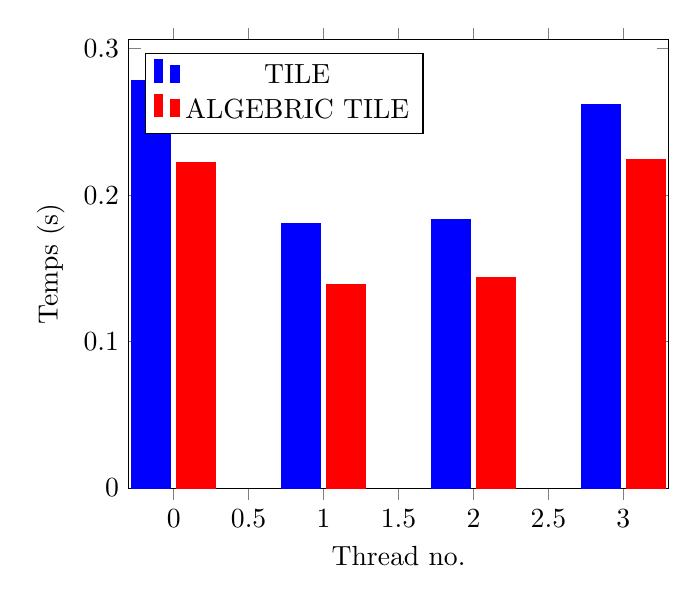
\begin{tikzpicture}
    \begin{axis}[
      ybar,
      bar width=0.5cm,
      xlabel={Thread no.},
      ylabel={Temps (s)},
      ymin=0,
      legend pos=north west
    ]

    % Données pour gemm.c
    \addplot[color=blue, fill=blue] coordinates {
      (0,0.278270) (1,0.180709) (2,0.183419) (3,0.261867)
    };
    \addlegendentry{TILE}

    \addplot[color=red, fill=red] coordinates {
      (0,0.222315) (1,0.138619) (2,0.143442) (3,0.224572)
    };
    \addlegendentry{ALGEBRIC TILE}

    \end{axis}
  \end{tikzpicture}
  \caption{Temps d'exécution des threads pour le fichier gemm.c}
  \label{fig:gemm.c}
\end{figure}

\begin{table}[htbp]
  \centering
  \caption{Statistiques pour le fichier gemm.c}
  \begin{tabular}{|c|c|c|}
    \hline
    Statistique & Algebraic Tile & Tile \\ 
    \hline
    Skewness (g1) & -0.00399974 & 0.0493613 \\ 
    Kurtosis (g2) & -1.99168 & -1.93083 \\ 
    Écart type & 0.0443931 & 0.0443931 \\ 
    Percent Imbalance metric en \% & 23.0924 & 23.0924 \\ 
    Temps d'exécution (s) &  0.224574      &  0.278277    \\ 
    \hline
  \end{tabular}
\end{table}
\newpage

\begin{figure}
  \centering
  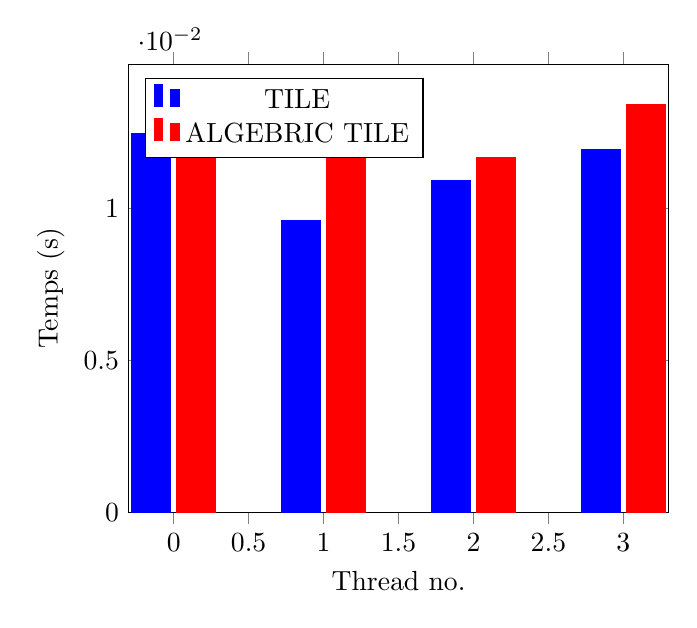
\begin{tikzpicture}
    \begin{axis}[
      ybar,
      bar width=0.5cm,
      xlabel={Thread no.},
      ylabel={Temps (s)},
      ymin=0,
      legend pos=north west
    ]

    % Données pour gemver.c
    \addplot[color=blue, fill=blue] coordinates {
      (0,0.012460) (1,0.009588) (2,0.010931) (3,0.011927)
    };
    \addlegendentry{TILE}

    \addplot[color=red, fill=red] coordinates {
      (0,0.013404) (1,0.011759) (2,0.011682) (3,0.013405)
    };
    \addlegendentry{ALGEBRIC TILE}

    \end{axis}
  \end{tikzpicture}
  \caption{Temps d'exécution des threads pour le fichier gemver.c}
  \label{fig:gemver.c}
\end{figure}

\begin{table}[htbp]
  \centering
  \caption{Statistiques pour le fichier gemver.c}
  \begin{tabular}{|c|c|c|}
    \hline
    Statistique & Algebraic Tile & Tile \\ 
    \hline
    Skewness (g1) & -0.00313065 & -0.421258 \\ 
    Kurtosis (g2) & -1.99583 & -1.29245 \\ 
    Écart type & 0.00109364 & 0.00109364 \\ 
    Percent Imbalance metric en \% & 10.9874 & 10.9874 \\ 
    Temps d'exécution (s) &  0.013427      &  0.012467    \\ 
    \hline
  \end{tabular}
\end{table}
\newpage

\begin{figure}
  \centering
  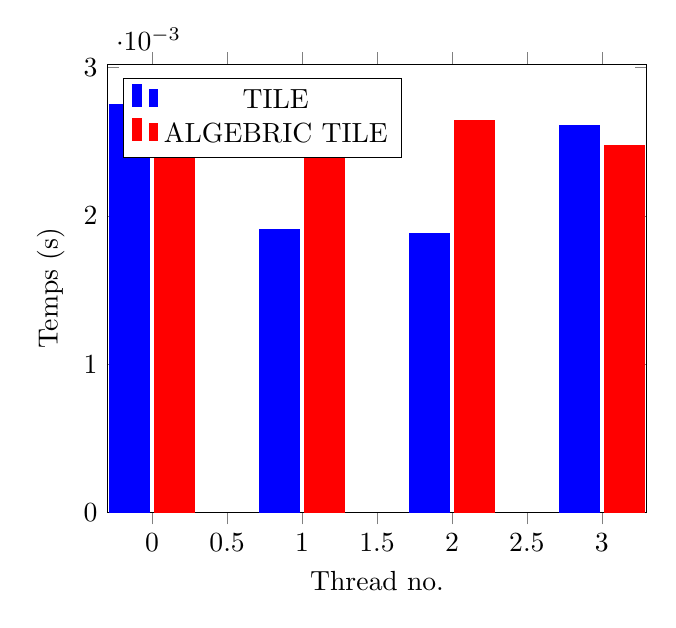
\begin{tikzpicture}
    \begin{axis}[
      ybar,
      bar width=0.5cm,
      xlabel={Thread no.},
      ylabel={Temps (s)},
      ymin=0,
      legend pos=north west
    ]

    % Données pour gesummv.c
    \addplot[color=blue, fill=blue] coordinates {
      (0,0.002749) (1,0.001910) (2,0.001882) (3,0.002607)
    };
    \addlegendentry{TILE}

    \addplot[color=red, fill=red] coordinates {
      (0,0.002459) (1,0.002642) (2,0.002643) (3,0.002476)
    };
    \addlegendentry{ALGEBRIC TILE}

    \end{axis}
  \end{tikzpicture}
  \caption{Temps d'exécution des threads pour le fichier gesummv.c}
  \label{fig:gesummv.c}
\end{figure}

\begin{table}[htbp]
  \centering
  \caption{Statistiques pour le fichier gesummv.c}
  \begin{tabular}{|c|c|c|}
    \hline
    Statistique & Algebraic Tile & Tile \\ 
    \hline
    Skewness (g1) & -0.0140065 & 0.0463413 \\ 
    Kurtosis (g2) & -1.98122 & -1.93353 \\ 
    Écart type & 0.000394334 & 0.000394334 \\ 
    Percent Imbalance metric en \% & 20.2011 & 20.2011 \\ 
    Temps d'exécution (s) &  0.002712      &  0.002756    \\ 
    \hline
  \end{tabular}
\end{table}
\newpage

\begin{figure}
  \centering
  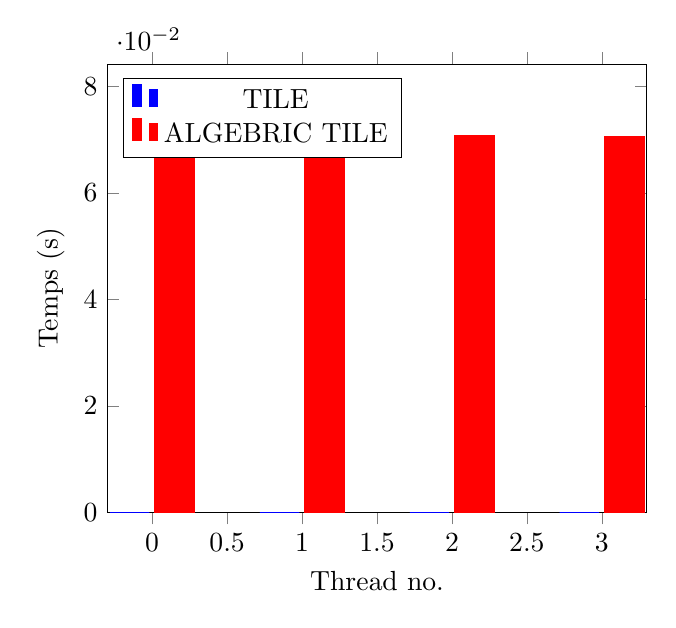
\begin{tikzpicture}
    \begin{axis}[
      ybar,
      bar width=0.5cm,
      xlabel={Thread no.},
      ylabel={Temps (s)},
      ymin=0,
      legend pos=north west
    ]

    % Données pour symm.c
    \addplot[color=blue, fill=blue] coordinates {
      (0,0.000000) (1,0.000000) (2,0.000000) (3,0.000000)
    };
    \addlegendentry{TILE}

    \addplot[color=red, fill=red] coordinates {
      (0,0.076532) (1,0.072543) (2,0.070738) (3,0.070637)
    };
    \addlegendentry{ALGEBRIC TILE}

    \end{axis}
  \end{tikzpicture}
  \caption{Temps d'exécution des threads pour le fichier symm.c}
  \label{fig:symm.c}
\end{figure}

\begin{table}[htbp]
  \centering
  \caption{Statistiques pour le fichier symm.c}
  \begin{tabular}{|c|c|c|}
    \hline
    Statistique & Algebraic Tile & Tile \\ 
    \hline
    Skewness (g1) & 0.844435 &  \\ 
    Kurtosis (g2) & -0.968908 &  \\ 
    Écart type & 0 & 0 \\ 
    Percent Imbalance metric en \% &  &  \\ 
    Temps d'exécution (s) &  1.178749      &  3.385856    \\ 
    \hline
  \end{tabular}
\end{table}
\newpage

\begin{figure}
  \centering
  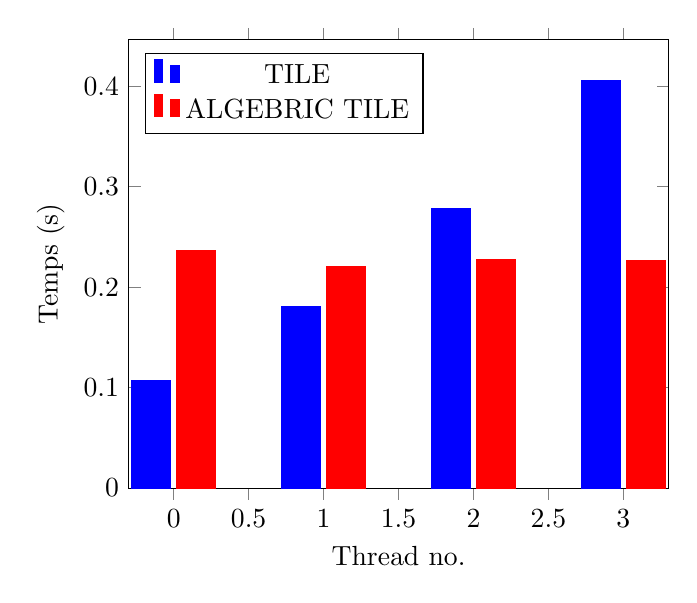
\begin{tikzpicture}
    \begin{axis}[
      ybar,
      bar width=0.5cm,
      xlabel={Thread no.},
      ylabel={Temps (s)},
      ymin=0,
      legend pos=north west
    ]

    % Données pour syr2k.c
    \addplot[color=blue, fill=blue] coordinates {
      (0,0.107359) (1,0.180932) (2,0.278325) (3,0.405563)
    };
    \addlegendentry{TILE}

    \addplot[color=red, fill=red] coordinates {
      (0,0.236194) (1,0.220163) (2,0.227023) (3,0.226485)
    };
    \addlegendentry{ALGEBRIC TILE}

    \end{axis}
  \end{tikzpicture}
  \caption{Temps d'exécution des threads pour le fichier syr2k.c}
  \label{fig:syr2k.c}
\end{figure}

\begin{table}[htbp]
  \centering
  \caption{Statistiques pour le fichier syr2k.c}
  \begin{tabular}{|c|c|c|}
    \hline
    Statistique & Algebraic Tile & Tile \\ 
    \hline
    Skewness (g1) & 0.367214 & 0.286622 \\ 
    Kurtosis (g2) & -0.974022 & -1.31019 \\ 
    Écart type & 0.11172 & 0.11172 \\ 
    Percent Imbalance metric en \% & 66.8675 & 66.8675 \\ 
    Temps d'exécution (s) &  0.236199      &  0.405662    \\ 
    \hline
  \end{tabular}
\end{table}
\newpage

\begin{figure}
  \centering
  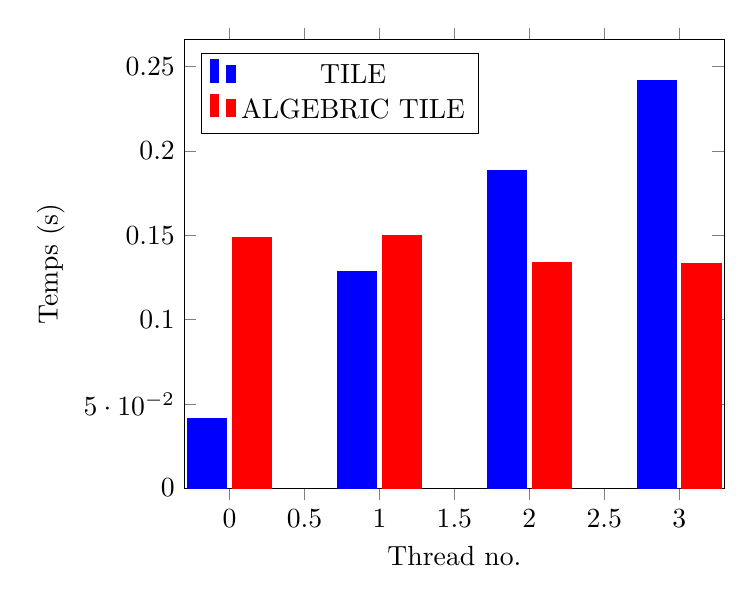
\begin{tikzpicture}
    \begin{axis}[
      ybar,
      bar width=0.5cm,
      xlabel={Thread no.},
      ylabel={Temps (s)},
      ymin=0,
      legend pos=north west
    ]

    % Données pour syrk.c
    \addplot[color=blue, fill=blue] coordinates {
      (0,0.041339) (1,0.128331) (2,0.188351) (3,0.241823)
    };
    \addlegendentry{TILE}

    \addplot[color=red, fill=red] coordinates {
      (0,0.148888) (1,0.150088) (2,0.133813) (3,0.133438)
    };
    \addlegendentry{ALGEBRIC TILE}

    \end{axis}
  \end{tikzpicture}
  \caption{Temps d'exécution des threads pour le fichier syrk.c}
  \label{fig:syrk.c}
\end{figure}

\begin{table}[htbp]
  \centering
  \caption{Statistiques pour le fichier syrk.c}
  \begin{tabular}{|c|c|c|}
    \hline
    Statistique & Algebraic Tile & Tile \\ 
    \hline
    Skewness (g1) & 0.00770974 & -0.278504 \\ 
    Kurtosis (g2) & -1.98751 & -1.2695 \\ 
    Écart type & 0.0744631 & 0.0744631 \\ 
    Percent Imbalance metric en \% & 61.2573 & 61.2573 \\ 
    Temps d'exécution (s) &  0.150169      &  0.241925    \\ 
    \hline
  \end{tabular}
\end{table}
\newpage

\begin{figure}
  \centering
  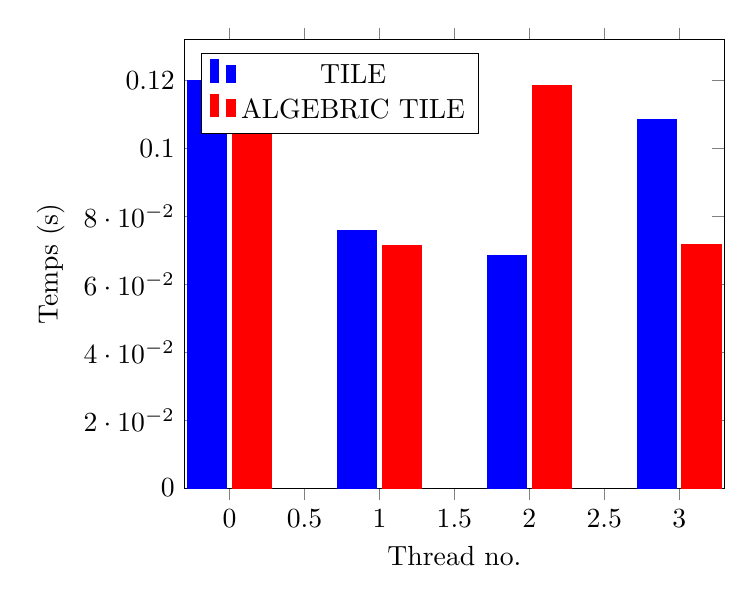
\begin{tikzpicture}
    \begin{axis}[
      ybar,
      bar width=0.5cm,
      xlabel={Thread no.},
      ylabel={Temps (s)},
      ymin=0,
      legend pos=north west
    ]

    % Données pour trmm.c
    \addplot[color=blue, fill=blue] coordinates {
      (0,0.119992) (1,0.075959) (2,0.068446) (3,0.108498)
    };
    \addlegendentry{TILE}

    \addplot[color=red, fill=red] coordinates {
      (0,0.115651) (1,0.071412) (2,0.118363) (3,0.071698)
    };
    \addlegendentry{ALGEBRIC TILE}

    \end{axis}
  \end{tikzpicture}
  \caption{Temps d'exécution des threads pour le fichier trmm.c}
  \label{fig:trmm.c}
\end{figure}

\begin{table}[htbp]
  \centering
  \caption{Statistiques pour le fichier trmm.c}
  \begin{tabular}{|c|c|c|}
    \hline
    Statistique & Algebraic Tile & Tile \\ 
    \hline
    Skewness (g1) & 0.00526667 & 0.0593975 \\ 
    Kurtosis (g2) & -1.99282 & -1.8073 \\ 
    Écart type & 0.0215746 & 0.0215746 \\ 
    Percent Imbalance metric en \% & 28.7141 & 28.7141 \\ 
    Temps d'exécution (s) &  0.118367      &  0.120002    \\ 
    \hline
  \end{tabular}
\end{table}
\newpage

\begin{figure}
  \centering
  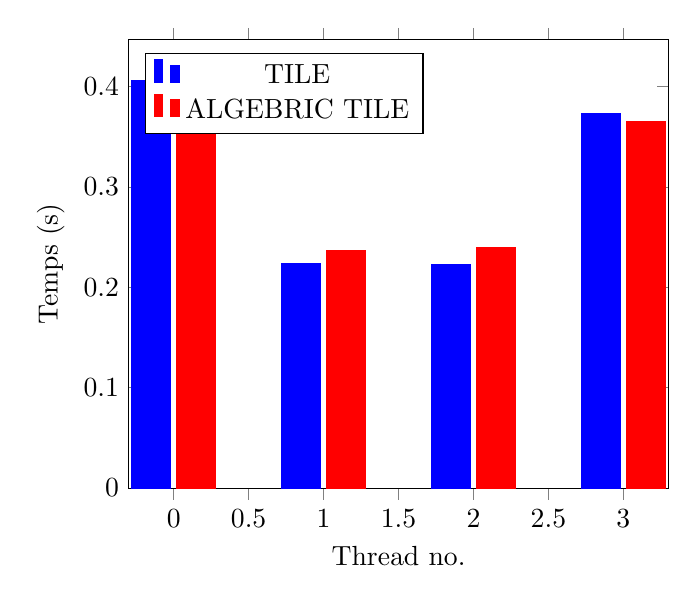
\begin{tikzpicture}
    \begin{axis}[
      ybar,
      bar width=0.5cm,
      xlabel={Thread no.},
      ylabel={Temps (s)},
      ymin=0,
      legend pos=north west
    ]

    % Données pour 2mm.c
    \addplot[color=blue, fill=blue] coordinates {
      (0,0.405934) (1,0.223307) (2,0.223058) (3,0.373408)
    };
    \addlegendentry{TILE}

    \addplot[color=red, fill=red] coordinates {
      (0,0.365331) (1,0.237018) (2,0.239464) (3,0.365025)
    };
    \addlegendentry{ALGEBRIC TILE}

    \end{axis}
  \end{tikzpicture}
  \caption{Temps d'exécution des threads pour le fichier 2mm.c}
  \label{fig:2mm.c}
\end{figure}

\begin{table}[htbp]
  \centering
  \caption{Statistiques pour le fichier 2mm.c}
  \begin{tabular}{|c|c|c|}
    \hline
    Statistique & Algebraic Tile & Tile \\ 
    \hline
    Skewness (g1) & -0.000548093 & 0.0556472 \\ 
    Kurtosis (g2) & -1.99925 & -1.92614 \\ 
    Écart type & 0.0840348 & 0.0840348 \\ 
    Percent Imbalance metric en \% & 32.4733 & 32.4733 \\ 
    Temps d'exécution (s) &  0.365906      &  0.405943    \\ 
    \hline
  \end{tabular}
\end{table}
\newpage

\begin{figure}
  \centering
  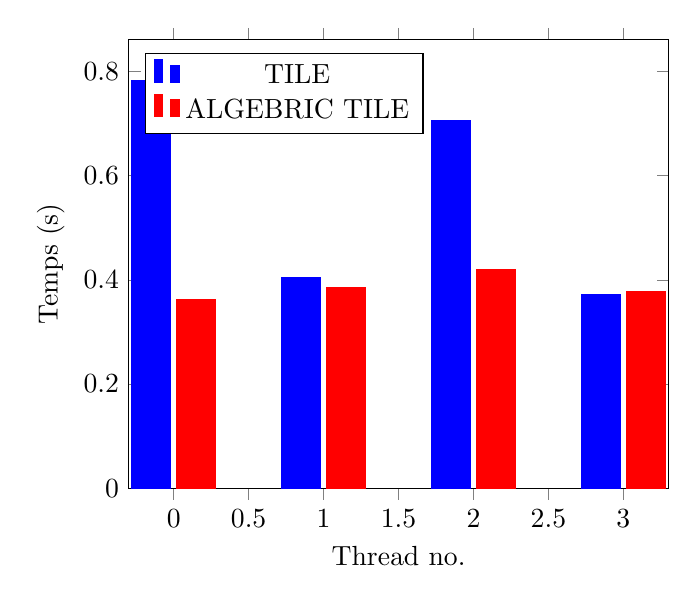
\begin{tikzpicture}
    \begin{axis}[
      ybar,
      bar width=0.5cm,
      xlabel={Thread no.},
      ylabel={Temps (s)},
      ymin=0,
      legend pos=north west
    ]

    % Données pour 3mm.c
    \addplot[color=blue, fill=blue] coordinates {
      (0,0.782972) (1,0.403797) (2,0.706874) (3,0.371239)
    };
    \addlegendentry{TILE}

    \addplot[color=red, fill=red] coordinates {
      (0,0.362432) (1,0.384658) (2,0.419438) (3,0.378208)
    };
    \addlegendentry{ALGEBRIC TILE}

    \end{axis}
  \end{tikzpicture}
  \caption{Temps d'exécution des threads pour le fichier 3mm.c}
  \label{fig:3mm.c}
\end{figure}

\begin{table}[htbp]
  \centering
  \caption{Statistiques pour le fichier 3mm.c}
  \begin{tabular}{|c|c|c|}
    \hline
    Statistique & Algebraic Tile & Tile \\ 
    \hline
    Skewness (g1) & 0.632198 & 0.0533916 \\ 
    Kurtosis (g2) & -0.948957 & -1.89794 \\ 
    Écart type & 0.181083 & 0.181083 \\ 
    Percent Imbalance metric en \% & 38.2803 & 38.2803 \\ 
    Temps d'exécution (s) &  0.428802      &  0.782992    \\ 
    \hline
  \end{tabular}
\end{table}
\newpage

\begin{figure}
  \centering
  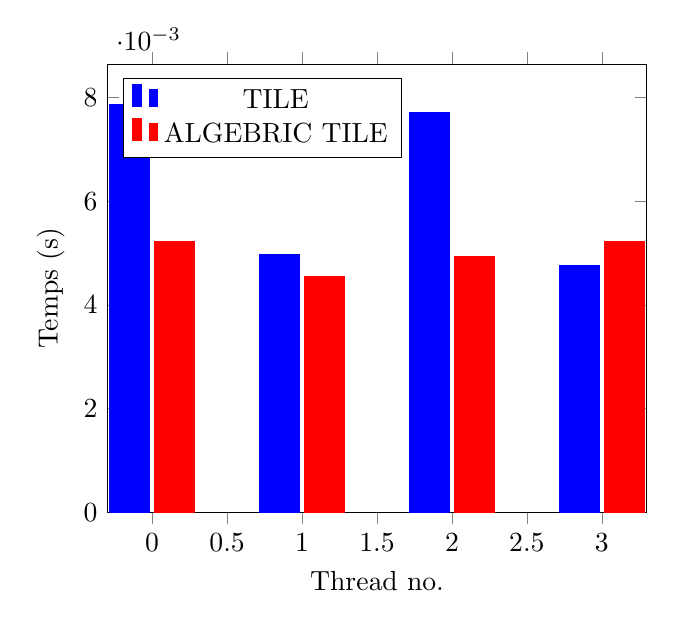
\begin{tikzpicture}
    \begin{axis}[
      ybar,
      bar width=0.5cm,
      xlabel={Thread no.},
      ylabel={Temps (s)},
      ymin=0,
      legend pos=north west
    ]

    % Données pour atax.c
    \addplot[color=blue, fill=blue] coordinates {
      (0,0.007858) (1,0.004983) (2,0.007707) (3,0.004766)
    };
    \addlegendentry{TILE}

    \addplot[color=red, fill=red] coordinates {
      (0,0.005226) (1,0.004544) (2,0.004942) (3,0.005232)
    };
    \addlegendentry{ALGEBRIC TILE}

    \end{axis}
  \end{tikzpicture}
  \caption{Temps d'exécution des threads pour le fichier atax.c}
  \label{fig:atax.c}
\end{figure}

\begin{table}[htbp]
  \centering
  \caption{Statistiques pour le fichier atax.c}
  \begin{tabular}{|c|c|c|}
    \hline
    Statistique & Algebraic Tile & Tile \\ 
    \hline
    Skewness (g1) & -0.651733 & -0.00428162 \\ 
    Kurtosis (g2) & -1.18466 & -1.9836 \\ 
    Écart type & 0.001457 & 0.001457 \\ 
    Percent Imbalance metric en \% & 24.1684 & 24.1684 \\ 
    Temps d'exécution (s) &  0.005374      &  0.007873    \\ 
    \hline
  \end{tabular}
\end{table}
\newpage

\begin{figure}
  \centering
  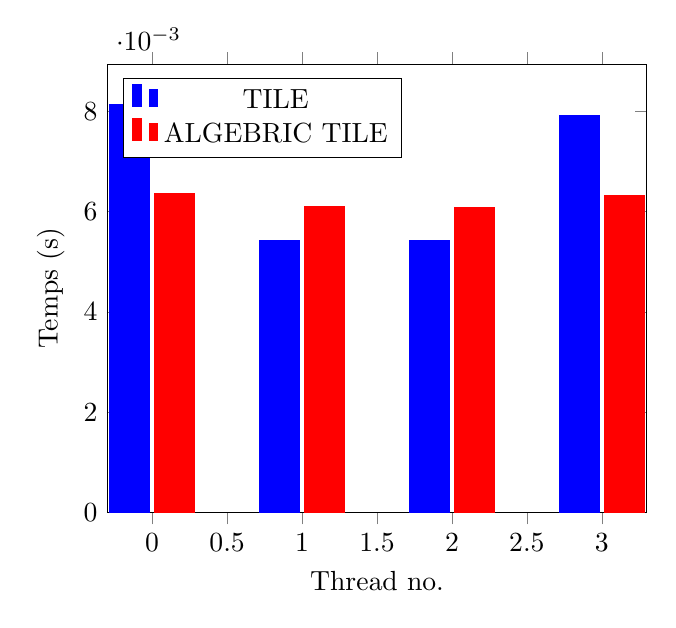
\begin{tikzpicture}
    \begin{axis}[
      ybar,
      bar width=0.5cm,
      xlabel={Thread no.},
      ylabel={Temps (s)},
      ymin=0,
      legend pos=north west
    ]

    % Données pour bicg.c
    \addplot[color=blue, fill=blue] coordinates {
      (0,0.008123) (1,0.005413) (2,0.005419) (3,0.007903)
    };
    \addlegendentry{TILE}

    \addplot[color=red, fill=red] coordinates {
      (0,0.006356) (1,0.006104) (2,0.006074) (3,0.006318)
    };
    \addlegendentry{ALGEBRIC TILE}

    \end{axis}
  \end{tikzpicture}
  \caption{Temps d'exécution des threads pour le fichier bicg.c}
  \label{fig:bicg.c}
\end{figure}

\begin{table}[htbp]
  \centering
  \caption{Statistiques pour le fichier bicg.c}
  \begin{tabular}{|c|c|c|}
    \hline
    Statistique & Algebraic Tile & Tile \\ 
    \hline
    Skewness (g1) & 0.012897 & 0.0106988 \\ 
    Kurtosis (g2) & -1.92658 & -1.98573 \\ 
    Écart type & 0.00130083 & 0.00130083 \\ 
    Percent Imbalance metric en \% & 20.977 & 20.977 \\ 
    Temps d'exécution (s) &  0.006459      &  0.008133    \\ 
    \hline
  \end{tabular}
\end{table}
\newpage

\begin{figure}
  \centering
  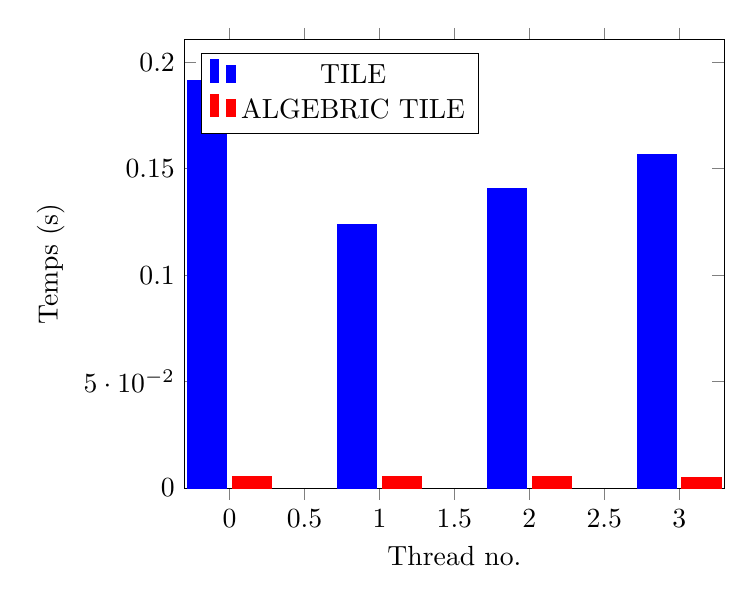
\begin{tikzpicture}
    \begin{axis}[
      ybar,
      bar width=0.5cm,
      xlabel={Thread no.},
      ylabel={Temps (s)},
      ymin=0,
      legend pos=north west
    ]

    % Données pour doitgen.c
    \addplot[color=blue, fill=blue] coordinates {
      (0,0.191459) (1,0.123812) (2,0.140476) (3,0.156500)
    };
    \addlegendentry{TILE}

    \addplot[color=red, fill=red] coordinates {
      (0,0.005183) (1,0.005360) (2,0.005343) (3,0.005169)
    };
    \addlegendentry{ALGEBRIC TILE}

    \end{axis}
  \end{tikzpicture}
  \caption{Temps d'exécution des threads pour le fichier doitgen.c}
  \label{fig:doitgen.c}
\end{figure}

\begin{table}[htbp]
  \centering
  \caption{Statistiques pour le fichier doitgen.c}
  \begin{tabular}{|c|c|c|}
    \hline
    Statistique & Algebraic Tile & Tile \\ 
    \hline
    Skewness (g1) & 0.00447622 & 0.474101 \\ 
    Kurtosis (g2) & -1.96899 & -1.1244 \\ 
    Écart type & 0.0250006 & 0.0250006 \\ 
    Percent Imbalance metric en \% & 25.0859 & 25.0859 \\ 
    Temps d'exécution (s) &  0.005415      &  0.247969    \\ 
    \hline
  \end{tabular}
\end{table}
\newpage

\begin{figure}
  \centering
  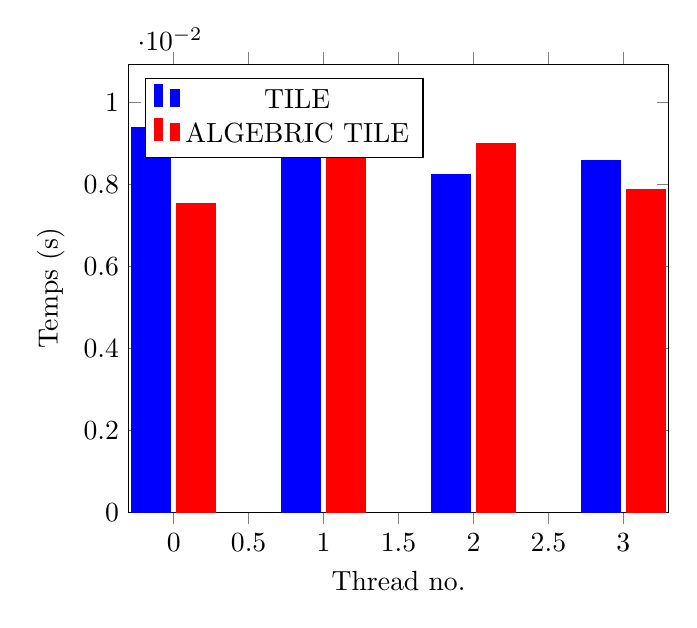
\begin{tikzpicture}
    \begin{axis}[
      ybar,
      bar width=0.5cm,
      xlabel={Thread no.},
      ylabel={Temps (s)},
      ymin=0,
      legend pos=north west
    ]

    % Données pour mvt.c
    \addplot[color=blue, fill=blue] coordinates {
      (0,0.009386) (1,0.009931) (2,0.008230) (3,0.008579)
    };
    \addlegendentry{TILE}

    \addplot[color=red, fill=red] coordinates {
      (0,0.007537) (1,0.009050) (2,0.008984) (3,0.007867)
    };
    \addlegendentry{ALGEBRIC TILE}

    \end{axis}
  \end{tikzpicture}
  \caption{Temps d'exécution des threads pour le fichier mvt.c}
  \label{fig:mvt.c}
\end{figure}

\begin{table}[htbp]
  \centering
  \caption{Statistiques pour le fichier mvt.c}
  \begin{tabular}{|c|c|c|}
    \hline
    Statistique & Algebraic Tile & Tile \\ 
    \hline
    Skewness (g1) & -0.0864067 & 0.138563 \\ 
    Kurtosis (g2) & -1.87633 & -1.58275 \\ 
    Écart type & 0.000667445 & 0.000667445 \\ 
    Percent Imbalance metric en \% & 9.95959 & 9.95959 \\ 
    Temps d'exécution (s) &  0.009054      &  0.009933    \\ 
    \hline
  \end{tabular}
\end{table}
\newpage

\begin{figure}
  \centering
  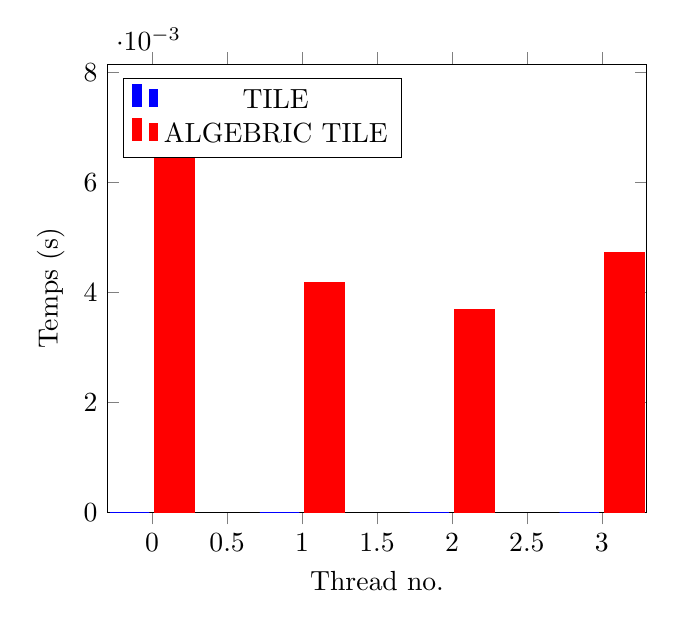
\begin{tikzpicture}
    \begin{axis}[
      ybar,
      bar width=0.5cm,
      xlabel={Thread no.},
      ylabel={Temps (s)},
      ymin=0,
      legend pos=north west
    ]

    % Données pour durbin.c
    \addplot[color=blue, fill=blue] coordinates {
      (0,0.000000) (1,0.000000) (2,0.000000) (3,0.000000)
    };
    \addlegendentry{TILE}

    \addplot[color=red, fill=red] coordinates {
      (0,0.007413) (1,0.004183) (2,0.003695) (3,0.004731)
    };
    \addlegendentry{ALGEBRIC TILE}

    \end{axis}
  \end{tikzpicture}
  \caption{Temps d'exécution des threads pour le fichier durbin.c}
  \label{fig:durbin.c}
\end{figure}

\begin{table}[htbp]
  \centering
  \caption{Statistiques pour le fichier durbin.c}
  \begin{tabular}{|c|c|c|}
    \hline
    Statistique & Algebraic Tile & Tile \\ 
    \hline
    Skewness (g1) & 0.936458 &  \\ 
    Kurtosis (g2) & -0.833167 &  \\ 
    Écart type & 0 & 0 \\ 
    Percent Imbalance metric en \% &  &  \\ 
    Temps d'exécution (s) &  0.012989      &  0.003360    \\ 
    \hline
  \end{tabular}
\end{table}
\newpage

\begin{figure}
  \centering
  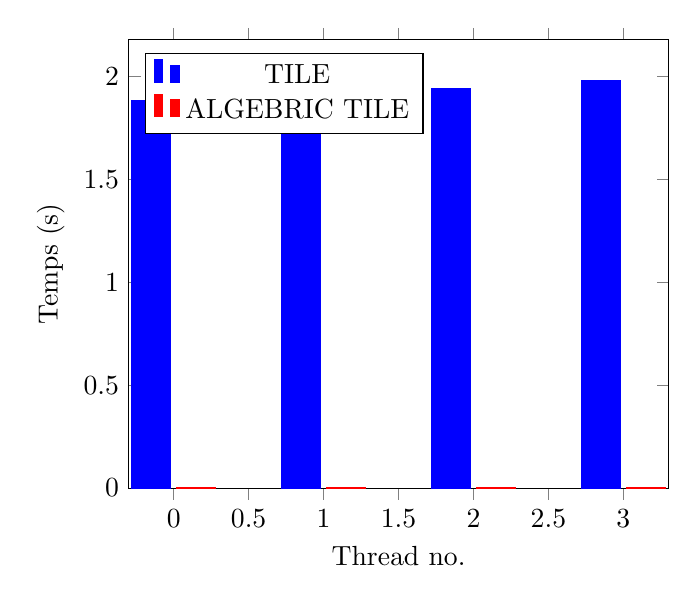
\begin{tikzpicture}
    \begin{axis}[
      ybar,
      bar width=0.5cm,
      xlabel={Thread no.},
      ylabel={Temps (s)},
      ymin=0,
      legend pos=north west
    ]

    % Données pour gramschmidt.c
    \addplot[color=blue, fill=blue] coordinates {
      (0,1.880755) (1,1.832727) (2,1.938989) (3,1.980397)
    };
    \addlegendentry{TILE}

    \addplot[color=red, fill=red] coordinates {
      (0,0.004655) (1,0.004099) (2,0.003809) (3,0.002644)
    };
    \addlegendentry{ALGEBRIC TILE}

    \end{axis}
  \end{tikzpicture}
  \caption{Temps d'exécution des threads pour le fichier gramschmidt.c}
  \label{fig:gramschmidt.c}
\end{figure}

\begin{table}[htbp]
  \centering
  \caption{Statistiques pour le fichier gramschmidt.c}
  \begin{tabular}{|c|c|c|}
    \hline
    Statistique & Algebraic Tile & Tile \\ 
    \hline
    Skewness (g1) & -0.571021 & -0.0645707 \\ 
    Kurtosis (g2) & -0.992678 & -1.46334 \\ 
    Écart type & 0.0561466 & 0.0561466 \\ 
    Percent Imbalance metric en \% & 3.78243 & 3.78243 \\ 
    Temps d'exécution (s) &  0.009210        &  2.217181    \\ 
    \hline
  \end{tabular}
\end{table}
\newpage

\begin{figure}
  \centering
  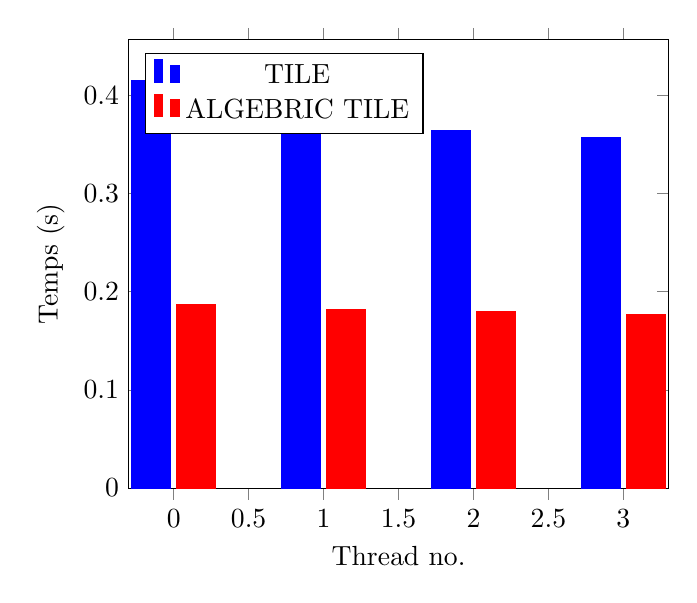
\begin{tikzpicture}
    \begin{axis}[
      ybar,
      bar width=0.5cm,
      xlabel={Thread no.},
      ylabel={Temps (s)},
      ymin=0,
      legend pos=north west
    ]

    % Données pour 2mm.c
    \addplot[color=blue, fill=blue] coordinates {
      (0,0.415226) (1,0.367814) (2,0.364741) (3,0.357203)
    };
    \addlegendentry{TILE}

    \addplot[color=red, fill=red] coordinates {
      (0,0.186935) (1,0.181784) (2,0.179524) (3,0.176917)
    };
    \addlegendentry{ALGEBRIC TILE}

    \end{axis}
  \end{tikzpicture}
  \caption{Temps d'exécution des threads pour le fichier 2mm.c}
  \label{fig:2mm.c}
\end{figure}

\begin{table}[htbp]
  \centering
  \caption{Statistiques pour le fichier 2mm.c}
  \begin{tabular}{|c|c|c|}
    \hline
    Statistique & Algebraic Tile & Tile \\ 
    \hline
    Skewness (g1) & 0.453558 & 1.05415 \\ 
    Kurtosis (g2) & -1.11664 & -0.735103 \\ 
    Écart type & 0.0228339 & 0.0228339 \\ 
    Percent Imbalance metric en \% & 10.3602 & 10.3602 \\ 
    Temps d'exécution (s) &  0.188175     &  0.415267    \\ 
    \hline
  \end{tabular}
\end{table}
\newpage

\begin{figure}
  \centering
  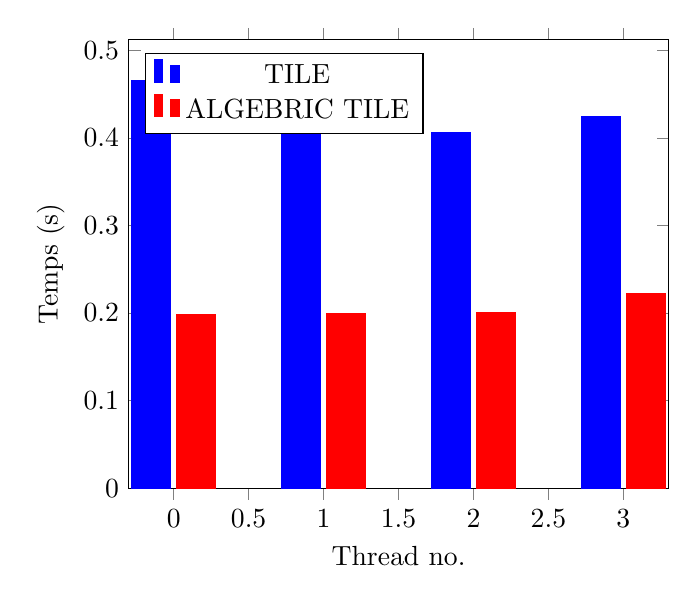
\begin{tikzpicture}
    \begin{axis}[
      ybar,
      bar width=0.5cm,
      xlabel={Thread no.},
      ylabel={Temps (s)},
      ymin=0,
      legend pos=north west
    ]

    % Données pour 2mm.c
    \addplot[color=blue, fill=blue] coordinates {
      (0,0.465589) (1,0.418188) (2,0.406051) (3,0.424091)
    };
    \addlegendentry{TILE}

    \addplot[color=red, fill=red] coordinates {
      (0,0.198066) (1,0.199656) (2,0.201006) (3,0.222395)
    };
    \addlegendentry{ALGEBRIC TILE}

    \end{axis}
  \end{tikzpicture}
  \caption{Temps d'exécution des threads pour le fichier 2mm.c}
  \label{fig:2mm.c}
\end{figure}

\begin{table}[htbp]
  \centering
  \caption{Statistiques pour le fichier 2mm.c}
  \begin{tabular}{|c|c|c|}
    \hline
    Statistique & Algebraic Tile & Tile \\ 
    \hline
    Skewness (g1) & 1.11673 & 0.860702 \\ 
    Kurtosis (g2) & -0.695334 & -0.850422 \\ 
    Écart type & 0.0223904 & 0.0223904 \\ 
    Percent Imbalance metric en \% & 8.66061 & 8.66061 \\ 
    Temps d'exécution (s) &  0.222832 &  0.465638    \\ 
    \hline
  \end{tabular}
\end{table}
\newpage

  \end{document}
